%%%%%%%%%%%%%%%%%%%%%%%%%%%%%%%%%%%%%%%%%%%%%%%%%%%%%%%%%%%%%%%%%%%%%%%%%%%%%%%
%
%  colloid.tex
%
%%%%%%%%%%%%%%%%%%%%%%%%%%%%%%%%%%%%%%%%%%%%%%%%%%%%%%%%%%%%%%%%%%%%%%%%%%%%%%%

\section{Colloids}


\subsection{General}

Colloidal particles are assumed to be spherical with a geometrical
centre $\mathbf{r}_c$, which is also the centre of mass. The
centre is allowed to move continuously across the lattice
with velocity $\mathbf{U}$; the particle has an angular velocity
$\mathbf{\Omega}$. The surface of the colloid is defined by an
input radius, $a_0$, which determines which lattice nodes are
inside or outside the colloid. (The hydrodynamic properties of
the colloid are specified by a different radius $a_h$ --- more
of this later.) The boundary links are then the set of vectors
joining lattice nodes which intersect the spherical surface
$\{\mathbf{c}_b\}$. A schematic picture is presented in
Figure~\ref{fig_coll2}. Note that a lattice node exactly at
the solid-fluid interface is defined to be outside the colloid.

In the original approach of Ladd, fluid occupied nodes both inside
and outside the particle. The effect of the ``internal fluid'' is
known to be restricted to short time scales (compared to the
characteristic time $a_0^2/\nu$), on which the fluid inside the
particle relaxes to a solid body rotation \cite{heemels}. There
are a number of problems related to the internal fluid, so we
use fully solid particles.

Nguyen and Ladd.

For each boundary link, it is useful to define a boundary vector,
$\mathbf{r}_b$, which connects the centre of the colloid to the
appropriate boundary node (note that the length of this vector is
not necessarily equal to the input radius of the colloid).


\begin{figure}[tb]
\begin{center}
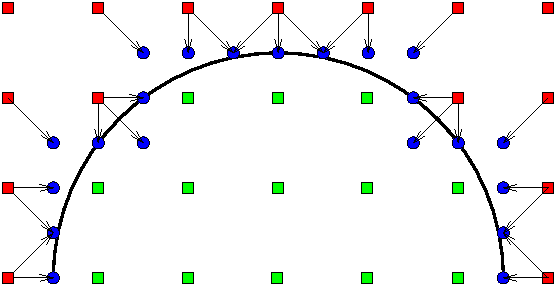
\includegraphics{xfig/colloidhalflinksnew-eps-converted-to.pdf}
\end{center}
\caption{Boundary links for a colloidal particle in two dimensions
with D2Q9 (half the particle is shown). Links join fluid sites (red)
to solid sites (green) and
intersect the circular shell radius $a_0$. Boundary nodes (circles)
lie exactly half way between pairs of lattice nodes. The generalisation
to three dimensions is straightforward.}
\label{fig_coll2}
\end{figure}

A \textit{boundary node} halfway between fluid nodes which are joined
by a boundary link. The position of the boundary node is always
exactly halfway along the boundary link ($\mathbf{r} + \frac{1}{2}\mathbf{c}_b
\Delta t$) regardless of the actual position of the intersection
of the colloid surface and the boundary link.
The colloid therefore has a discrete representation which becomes a
better approximation to the sphere as the input radius becomes larger;
this approximation is known to be reasonably good for $a_0 > 5\Delta x$.



\subsection{Bounce-back on links}

The standard boundary condition required for the solid-fluid
interface of a moving particle is described by Ladd \cite{l94b},
and is generally refered to as bounce-back on links (BBL).
A boundary link is defined as joining a node $\mathbf{r}$
inside the particle to one outside at $\mathbf{r} + \mathbf{c}_b \Delta t$.
If the post-collision distributions are denoted by $f^\ast$, then
the distributions must be reflected at the solid surface so that
\begin{equation}
\label{eq:bbl1}
f_{b'}(\mathbf{r}; t + \Delta t) = f_b^\ast (\mathbf{r}; t)
- \frac{2w_{c_b} \rho \mathbf{u}_b.\mathbf{c}_b}{c_s^2}
\end{equation}
where the boundary link $\mathbf{c}_{b'} = -\mathbf{c}_b$. The velocity
at the boundary
\begin{equation}
\label{eq:ub}
\mathbf{u}_b = \mathbf{U} + \mathbf{\Omega}\times\mathbf{r}_b
\end{equation}
is determined by the particle linear velocity $\mathbf{U}$ and angular
velocity $\mathbf{\Omega}$. The change in momentum described by

The force exerted on a
single link is
\begin{equation}
\mathbf{F}_b(\mathbf{r} + {\scriptstyle\frac{1}{2}}\mathbf{c}_b\Delta t;
t + {\scriptstyle\frac{1}{2}}\Delta t) = \frac{\Delta x^3}{\Delta t}
\Big[ 2f_b^\ast(\mathbf{r}; t) - \frac{2w_{c_b}\rho_0 \mathbf{u}_b .
\mathbf{c}_b}{c_s^2} \Big] \mathbf{c}_b,
\label{eq:fb}
\end{equation}
with corresponding torque $\mathbf{T}_b = \mathbf{r}_b \times \mathbf{F}_b$.




The total hydrodynamic force on the particle is then found by taking
the sum of
$\mathbf{F}_b$ over all the boundary links defining the particle.
The is an associated torque on each link of $\mathbf{r}_b\times\mathbf{F}_b$,
which again is summed over all links to give the total torque on the colloid.

Note that $\rho$ in the above equations is the density of the fluid
at the appropriate fluid node for the link. As the density fluctuations
in the fluid are small compared with the mean density $\rho_0$, the
density in the correction to the bounce-back can be replaced by the
mean $\rho_0$.


\subsection{Dynamics}
Having computed the total force and torque on an individual colloid,
is is possible to update the the linear velocities
\begin{equation}
m_0 \mathbf{U}(t + \Delta t) = m_0 \mathbf{U}(t) + \Delta t \mathbf{F} (t),
\end{equation}
where the mass of the colloid is related to the input radius by
$m_0 = {\scriptstyle\frac{4}{3}}\pi\rho_0 a_0^3$ and the angular
velocity
\begin{equation}
I_0 \mathbf{\Omega} (t + \Delta t) = I_0 \mathbf{\Omega}(t) + \Delta t
\mathbf{T}(t),
\end{equation}
where the moment of inertia is $I_0 = {\scriptstyle\frac{2}{5}}m_o a_o^2$.
However, this explicit update is generally found to have poor stability
properties \cite{l94b, nl02}. The alternative is to use a velocity update
which is implicit \cite{heemels,nl02}.



The total force and torque on a colloid can be split into velocity-dependent
and -independent parts by combining Equations~(\ref{eq:ub})
and~(\ref{eq:fb}) to eliminate the boundary velocity $\mathbf{u}_b$.
In this way, the decomposition is
\begin{eqnarray}
\mathbf{F} = \mathbf{F}_0 - \boldsymbol{\zeta}^{FU}.\mathbf{U}
-\boldsymbol{\zeta}^{F\Omega}.\mathbf{\Omega},
\label{eq:d3}
\\
\mathbf{T} = \mathbf{T}_0 - \boldsymbol{\zeta}^{TU}.\mathbf{U}
-\boldsymbol{\zeta}^{T\Omega}.\mathbf{\Omega}.
\label{eq:d4}
\end{eqnarray}
The velocity independent parts of the force and the torque
(appropriate for a colloid at rest) are
\begin{eqnarray}
\mathbf{F}_0(t + {\scriptstyle\frac{1}{2}}\Delta t) =
\frac{2\Delta x^3}{\Delta t} \sum_b \big[ f_b^\ast(\mathbf{r}; t)
- f_{b'}^\ast(\mathbf{r} + \mathbf{c}_i \Delta t; t) \big] \mathbf{c}_b,
\\
\mathbf{T}_0(t + {\scriptstyle\frac{1}{2}}\Delta t) =
\frac{2\Delta x^3}{\Delta t} \sum_b \big[ f_b^\ast(\mathbf{r}; t)
- f_{b'}^\ast(\mathbf{r} + \mathbf{c}_i \Delta t; t) \big]
(\mathbf{r}_b\times \mathbf{c}_b)
\end{eqnarray}
The matrices $\boldsymbol{\zeta}$ are interpreted as drag
coefficients and can be written as
\begin{eqnarray}
\mathbf{\boldsymbol{\zeta}}^{FU} &=& \frac{4\rho_0 \Delta x^3}{c_s^2 \Delta t}
\sum_b w_{c_b} \mathbf{c}_b \mathbf{c}_b,
\\
\mathbf{\boldsymbol{\zeta}}^{F\Omega} &=&
\frac{4\rho_0 \Delta x^3}{c_s^2 \Delta t}
\sum_b w_{c_b} \mathbf{c}_b (\mathbf{r}_b \times \mathbf{c}_b),
\\
\mathbf{\boldsymbol{\zeta}}^{TU} &=& \frac{4\rho_0 \Delta x^3}{c_s^2 \Delta t}
\sum_b w_{c_b} (\mathbf{r}_b \times \mathbf{c}_b) \mathbf{c}_b,
\\
\mathbf{\boldsymbol{\zeta}}^{T\Omega} &=&
\frac{4\rho_0 \Delta x^3}{c_s^2 \Delta t}
\sum_b w_{c_b} (\mathbf{r}_b \times \mathbf{c}_b)
(\mathbf{r}_b \times \mathbf{c}_b).
\end{eqnarray}
As an example, the full form of the $\boldsymbol{\zeta}^{F\Omega}$ matrix is

\begin{equation}
\label{eq:k14}
\left( \begin{array}{rrr}
\sum_b c_{bx} (\mathbf{r}_b \times \mathbf{c}_b)_x &
\sum_b c_{bx} (\mathbf{r}_b \times \mathbf{c}_b)_y &
\sum_b c_{bx} (\mathbf{r}_b \times \mathbf{c}_b)_z \\

\sum_b c_{by} (\mathbf{r}_b \times \mathbf{c}_b)_x &
\sum_b c_{by} (\mathbf{r}_b \times \mathbf{c}_b)_y &
\sum_b c_{by} (\mathbf{r}_b \times \mathbf{c}_b)_z \\

\sum_b c_{bz} (\mathbf{r}_b \times \mathbf{c}_b)_x &
\sum_b c_{bz} (\mathbf{r}_b \times \mathbf{c}_b)_y &
\sum_b c_{bz} (\mathbf{r}_b \times \mathbf{c}_b)_z \\

\end{array} \right).
\end{equation}
If the particle has a symmetric distribution of boundary links (the
special case where the centre of mass is on a symmetry point of the
lattice) the $\boldsymbol{\zeta}^{FU}$ and
$\boldsymbol{\zeta}^{T\Omega}$ matrices are
diagonal, while the $\boldsymbol{\zeta}^{F\Omega}$
and $\boldsymbol{\zeta}^{TU}$ matrices are zero.

The velocity updates can now be rewritten using an
implicit update, which results in
\begin{eqnarray}
\label{eq:k15}
m_0 \mathbf{U}(t + \Delta t) = m_0 \mathbf{U}(t) + \Delta t
\big[ \mathbf{F}_0 (t + {\scriptstyle\frac{1}{2}}\Delta t)
- \boldsymbol{\zeta}^{FU} . \mathbf{U}(t + \Delta t)
- \boldsymbol{\zeta}^{F\Omega}.\mathbf{\Omega}(t + \Delta t) \big],
\\
\label{eq:k16}
I_0 \mathbf{\Omega} (t + \Delta t) = I_0 \mathbf{\Omega}(t) + \Delta t
\big[ \mathbf{T}_0(t + {\scriptstyle\frac{1}{2}} \Delta t)
- \boldsymbol{\zeta}^{TU} . \mathbf{U}(t + \Delta t)
- \boldsymbol{\zeta}^{T\Omega}. \mathbf{\Omega}(t + \Delta t) \big].
\end{eqnarray}
In general all the matrix elements are non-zero, in which case
equations~(\ref{eq:k15}) and~(\ref{eq:k16}) can be solved via a
6$\times$6 matrix inversion.

Finally, the position of the particle can be updated: an Euler
forward step is taken using the updated velocity
\begin{equation}
\mathbf{r} (t + \Delta t) = \mathbf{r} (t) + \Delta t\mathbf{U}(t + \Delta t)
\end{equation}


\subsection{Changes in particle shape}

One consequence is that the discrete shape of the particle fluctuates
as the colloid centre moves relative to the
lattice. This means that the size of the particle as seen by the
fluid changes despite the fact that the input radius of the colloid
is fixed.  However, these fluctuations are small for input radii
greater than about 5 lattice units \cite{l96a}. Furthermore, the
fluctuations may be greater for some input radii than others
\cite{nl02}.


In the standard approach, changes in the map of boundary links
are accomodated by the internal fluid. If the particle shape
changes so that an internal node is exposed, the internal fluid
at that site rejoins the fluid proper with the solid body momentum
(assuming the internal fluid is relaxed to solid-body rotation).
If a fluid node is covered by particle movement, then it simply
joins the internal fluid, and will relax to solid-body rotation.
Without internal fluid, changes in particle shape
in which fluid nodes are either covered or uncovered must be
accompanied by the removal or addition
of fluid with appropriate properties at the nodes in question.
It is essential that this
is done in a way which minimises the perturbation to the fluid
flow.


If a fluid node at $\mathbf{r}$ is covered by the movement of a
solid particle,
the fluid loses a mass $\rho(\mathbf{r}) \Delta x^3$, of which an excess
$\Delta M_c = (\rho(\mathbf{r}) - \rho_0)\Delta x^3$ must be replaced
explicitly so that
the overall mass density is unchanged. At the same time, the
colloid must assume the momentum lost by the fluid
$\Delta x^3 \sum_i f_i(\mathbf{r}) \mathbf{c}_i$.

Similarly, when a fluid node is exposed by particle movement,
fluid must be replaced with the appropriate distribution, density
and velocity. If the
new density is $\rho$ (to be determined by some method) then
the fluid gains an excess of mass $\Delta M_u = (\rho - \rho_0)
\Delta x^3$ which must be balanced elsewhere. If the new fluid
is assumed to have velocity $\mathbf{u}$ then the particle must
give up momentum $\Delta x^3 \rho\mathbf{u}$.

Following Nguyen and Ladd \cite{nl02}, these changes owing
to change in particle shape are implemented by added a small
correction to the bounce-back at the following time step.
The excess mass from a covered fluid site is redistributed over all the
boundary nodes by redefined the mometum transfer at bounce-back
\begin{equation}
f_{b'}(\mathbf{r}; t + \Delta t) = f_b^\ast (\mathbf{r}; t)
- \frac{2 w_{c_b} \rho_0 \mathbf{u}_b . \mathbf{c}_b}{c_s^2}
+ \frac{w_{c_b} \rho_0\Delta M_c }{A},
\label{eq:q1}
\end{equation}
where $A = \rho_0 \Delta x^3 \sum_b w_{c_b}$. The accompanying
force on the particle owing to the change in shape is then
that lost by the fluid plus the contributions from the final term
in (\ref{eq:q1}) summed over all the boundary links
\begin{equation}
\Delta \mathbf{F}_c = \frac{\Delta x^3}{\Delta t}\sum_{i} f_i \mathbf{c}_i
+ \frac{\Delta x^3}{\Delta t} \sum_b \frac{w_{c_b} \rho_0 \Delta M_c}{A}
\mathbf{c}_b.
\label{eq:q2}
\end{equation}

Note that for a closed surface,
$\sum_b w_{c_b}\mathbf{c}_b = 0$, and the second term on the right-hand
side of Eq.~(\ref{eq:q2}) is zero, i.e., the redistribution of mass
does not contribute to the net force and torque on the particle.
The corresponding change in torque is
\begin{equation}
\Delta \mathbf{T}_c = \frac{\Delta x^3}{\Delta t} \mathbf{r}_c
\times \sum_i f_i \mathbf{c}_i
+ \frac{\Delta x^3}{\Delta t}
\sum_b \frac{w_{c_b}\rho_0 \Delta M_c}{A} \mathbf{r}_b \times \mathbf{c}_b,
\label{eq:q2a}
\end{equation}
where $\mathbf{r}_c$ is the boundary vector at the position where the
fluid has been removed. Again, for a closed surface, the
redistribution of mass does not contribute to the net torque
on the particle.

Likewise, the contribution to the bounce-back from newly uncovered nodes
is
\begin{equation}
- \frac{w_{c_b} \rho_0 \Delta M_u}{A}
\label{eq:q3}
\end{equation}
leading to a change in force of
\begin{equation}
\Delta \mathbf{F}_u = -\frac{\Delta x^3 \rho(\mathbf{r})
\mathbf{u}(\mathbf{r})}{\Delta t} - \frac{\Delta x^3}{\Delta t} \sum_b
\frac{w_{c_b} \rho_0 \Delta M_u}{A} \mathbf{c}_b,
\label{eq:q4}
\end{equation}
with a corresponding change in the torque.
If more than one lattice node is either covered or uncovered by
the movement of the particle, then these contributions add in a simple
way. The overall contributions can be added to the
velocity-independent terms $\mathbf{F}_0$ and $\mathbf{T}_0$ appearing in
Equations~(\ref{eq:d3}) and~(\ref{eq:d4}).



\subsection{Particles near contact}

Particles near contact may not pocess a full set of boundary
links (see Figure~\ref{fig:f5}). This leads to a potential
non-conservation of mass associated with the particle motion
which must be corrected.


\begin{figure}[tb]
\begin{center}
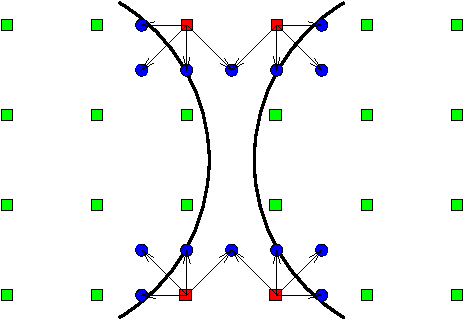
\includegraphics{xfig/colloidclose-eps-converted-to.pdf}
\end{center}
\caption{Two colloids close to contact are missing links in the
region of closest approach owing to a lack of fluid nodes in the
interstice.}
\label{fig:f5}
\end{figure}
Again following Nguyen and Ladd \cite{nl02}, mass conservation is
enforced explicitly using the following procedure. There is a mass
transfer associated with the bounce-back at each link of
$(2w_{c_b}\rho_0 \mathbf{u}_b . \mathbf{c}_b / c_s^2) \Delta x^3$.
The net mass transport into the particle is the sum of this
quantity over all the links, and can be written
\begin{equation}
\Delta M_s = - \frac{2\Delta x^3 \rho_0}{c_s^2}
\Big[ \mathbf{U}.\sum_b w_{c_b} \mathbf{c}_b +
  \mathbf{\Omega} . \sum_b w_{c_b} \mathbf{r}_b \times \mathbf{c}_b \Big].
\end{equation}
For any partilce with a full set of boundary links, both
$\sum_b w_{c_b} \mathbf{c}_b$
and $\sum_b w_{c_b} \mathbf{r}_b \times \mathbf{c}_b$ are zero.
However, if the set of boundary links is imcomplete
(as in Figure~\ref{fig:f5}) $\Delta M_s$ is not zero and
a correction is required. This is again made by redistributing the
excess or deficit of mass over the other existing boundary nodes.
The additional contribution to the bounce-back here is
$-w_{c_b} \rho_0 \Delta M_s/A$, where
$A = \rho_0 \Delta x^3 \sum_b w_{c_b}$ (cf.\ Equation~\ref{eq:q1}).

This contribution
now adds to the velocity-dependent part of the force and torque and
leads to a slightly different form of the drag matrices
\begin{eqnarray}
\boldsymbol{\zeta}^{FU} &=& \frac{-2\rho_0 \Delta x^3}{c_s^2 \Delta t}
\sum_b w_{c_b} (\mathbf{c}_b - \overline{\mathbf{c}_b}) \mathbf{c}_b
\\
\boldsymbol{\zeta}^{F\Omega} &=& \frac{-2\rho_0 \Delta x^3}{c_s^2 \Delta t}
\sum_b w_{c_b} \mathbf{c}_b (\mathbf{r}_b \times \mathbf{c}_b -
\overline{\mathbf{r}_b\times\mathbf{c}_b}),
\\
\boldsymbol{\zeta}^{TU} &=& \frac{-2\rho_0 \Delta x^3}{c_s^2 \Delta t}
\sum_b w_{c_b} (\mathbf{r}_b\times\mathbf{c}_b)
(\mathbf{c}_b - \overline{\mathbf{c}_b}),
\\
\boldsymbol{\zeta}^{T\Omega} &=& \frac{-2\rho_0 \Delta x^3}{c_s^2 \Delta t}
\sum_b w_{c_b} (\mathbf{r}_b\times\mathbf{c}_b)
(\mathbf{r}_b\times\mathbf{c}_b - \overline{\mathbf{r}_b\times\mathbf{c}_b}).
\end{eqnarray}
The mean quantities
\begin{equation}
\overline{\mathbf{c}_b} = \frac{\sum_b w_{c_b} \mathbf{c}_b}{ \sum_b w_{c_b}}
\end{equation}
and
\begin{equation}
\overline{\mathbf{r}_b\times\mathbf{c}_b} =
\frac{\sum_b w_{c_b} \mathbf{r}_b\times\mathbf{c}_b}{\sum_b w_{c_b}}.
\end{equation}
A little algebra will show that both occurances of $\mathbf{c}_b$ and/or
$\mathbf{r}_b\times\mathbf{c}_b$ in the definition of the drag matrices
can be replaced by their deviation from the mean. This provides a
convenient way to compute the drag matrices (maintaining symmetry)
and computing the correct force and torque on the particle when close
to contact.



\subsection{Rotational motions}


For a number of applications it is useful to update not only
the psoition of a spherical particle, but its orientation. This
is important, e.g., when considering magnetic particles. The
best way to implementment the required rotations is by
considering quaternions.

A quaternion can be thought of as an extended complex number
\begin{equation}
q = w + xi + yj + zk
\end{equation}
where $i^2 = j^2 = k^2 = -1$ and $ijk = -1$. The norm, or length
of a quaternion is
\begin{equation}
N(q) = (w^2 + x^2 + y^2 + z^2)^{1/2}.
\end{equation}
Addition and subtraction of quaternions proceeds as normal, but
care is required for multiplication, which is associative but not
commutative. If the quaternion is writen as $q = (w, {\bf v})$ where
$\bf{v}$ is a normal 3-vector, then multiplication can be written
\begin{equation}
q_1 q_2 = (w_1 w_2 - {\bf v}_1 . {\bf v}_2, w_1 {\bf v}_2 + w_2 {\bf v}_1
+ {\bf v}_1 \times {\bf v}_2),
\end{equation}
where the usual scalar and vector products are used. Note that the
conjugate of a quaterion $q^\star = (w, -{\bf v})$ so that
$qq^\star = N^2(q)$.
It can be shown that a rotation of an arbitrary vector though an
angle $\theta$ around the unit axis of rotaion $\hat{\bf w}$ can
be represented by the quarternion
\begin{equation}
q = (\cos(\theta/2), \hat{\bf w} \sin(\theta/2))
\end{equation}
which ensures that $N(q) = 1$. If the arbitrary vector is (0, {\bf v}),
then the rotated vector ${\bf v}^{'}$ can be written as
\begin{equation}
(0, {\bf v}^{'}) = q (0, {\bf v}) q^\star
\end{equation}
which can be expanded as
\begin{equation}
{\bf v}^{'} = (1 - \cos\theta)({\bf v}.{\hat{\bf w}) \hat{\bf w} +
{\bf v}\cos\theta} + (\hat{\bf w} \times {\bf v})\sin\theta.  
\end{equation}


\subsection{Colloid-Colloid interactions}

\subsubsection{Lubrication corrections}

\subsubsection{Hard sphere interaction}

Particles do not overlap, i.e., there is always
a hard-sphere interaction which is a function of the separation $h$:
\begin{equation}
v^{hs}(h) = \left\{
\begin{array}{ll}
\infty & h \leq 0,\\
0   & h > 0.
\end{array} \right.
\end{equation}
The hard-sphere interaction does not give rise to a force.


\subsubsection{Soft-sphere interaction}

A simple soft-sphere interaction is available, the basic form
of which is:
\begin{equation}
v^{ss}(r) = \epsilon (\sigma / r)^{\nu},
\end{equation}
where $\epsilon$ sets the energy scale, and $\sigma$ sets the
characteristic width. The steepness of the potential is set by
the exponent $\nu (> 0)$.

To prevent the need for calculation of long-range interactions,
the soft-sphere potential is truncated in a ``cut-and-shift''
approach. This is done in such a way as to smoothly match
both the potential and the force at the cut-off distance
$r_c$. For $r < r_c$ the potential is then
\begin{equation}
v^{ss}(r) - v^{ss}(r_c) - (r - r_c) \left.\frac{d v^{ss}}{dr}\right|_{r=r_c}.
\label{eq_ss_shift}
\end{equation}
Clearly, this potential is not exactly what we first thought of as
soft-sphere. Matching the potential smoothly ensures conservation
of energy, while matching the force smoothly prevents potential
instabilities in the molecular dynamics update.

The soft-sphere potential can be useful as a mechanism to
keep the particles from touching (which risks hard-sphere interactions),
in which case is is possible to compute the interaction as a function
of the separation $h$, instead of $r$. The force between
two particles is computed via the derivative of equation~\ref{eq_ss_shift}
with respect to $r$:
\begin{equation}
\mathbf{F}_{ij}(r) = -\left\{\frac{d v^{ss}(r)}{dr} -
\left. \frac{d v^{ss}(r)}{dr}\right|_{r=r_c} \right\} \mathbf{\hat{r}}_{ij}
\end{equation}
where $\mathbf{\hat{r}}_{ij}$ is the unit vector joining the centre of
particle $i$ to the centre of $j$.



\subsubsection{Leonard-Jones interaction}


\subsection{Cholesteric Anchoring}

We have a fluid free energy density
\begin{equation}
f = 
{\textstyle\frac{1}{2}} \kappa_0 (\partial_\beta Q_{\alpha\beta})^2
+ {\textstyle\frac{1}{2}}
 \kappa_1 (\epsilon_{\alpha\gamma\sigma} \partial_\gamma
Q_{\sigma\beta} + 2q_0 Q_{\alpha\beta})^2
\end{equation}
where we have ignored the bulk terms for the time being, but we retain
two elastic constants $\kappa_0$ and $\kappa_1$ in the distortion term.
The cholesteric pitch $p = 2\pi/q_0$.

There is also a surface term (an area density)
\begin{equation}
f_s = {\textstyle\frac{1}{2}} w_1 (Q_{\alpha\beta} - Q_{\alpha\beta}^0)^2
\end{equation}
where $Q^0_{\alpha\beta}$ is the preferred order parameter configuration
at the surface (in the case of normal anchoring or fixed planar anchoring).
For degenerate planar anchoring,
following Fournier and Galatola \cite{fournier2005}, we have
\begin{equation}
f_s = {\textstyle\frac{1}{2}} w_1 (\tilde{Q}_{\alpha\beta}
    - \tilde{Q}^\perp_{\alpha\beta})^2
    + {\textstyle\frac{1}{2}} w_2 (\tilde{Q}_{\alpha\beta}
                      \tilde{Q}_{\alpha\beta} - S^2_0)^2
\end{equation}
where $\tilde{Q}_{\alpha\beta} + (1/3)S_0 \delta_{\alpha\beta}$, $S_0$ is
is a fixed surface amplitude; to obtain a prefered degenerate
configuration we take the fluid order parameter $Q_{\alpha\beta}$ and
project $\tilde{Q}^\perp_{\alpha\beta} = P_{\alpha\gamma}
\tilde{Q}_{\gamma\sigma}
P_{\sigma\beta}$, where $P_{\alpha\beta} = \delta_{\alpha\beta}
- n_\alpha n_\beta$ and $n_\alpha$ is the local unit surface normal.

The boundary condition we wish to apply are the Euler-Lagrange equations. 
They are at the surface of the particle
\begin{equation}
n_\gamma \frac{\partial f}{\partial Q_{\alpha\beta,\gamma}} = 0
\end{equation}
where $Q_{\alpha\beta,\gamma} = \partial_\gamma Q_{\alpha\beta}$. Here,
$n_\gamma$ is the outward unit normal at the surface (pointing into the
fluid) \cite{skarabot}. Note that compared to the regular minimization as  
explained in \cite{wright} this is a surface integral term that would 
usually vanish in the bulk.
With the
addition of the surface term we obtain
\begin{equation}
n_\gamma \frac{\partial f}{\partial Q_{\alpha\beta,\gamma}}
+ \frac{\partial f_s}{\partial Q_{\alpha\beta}} = 0.
\end{equation}
The derivative of the distortion free energy with respect to
$Q_{\alpha\beta,\gamma}$ gives
\begin{equation}
\kappa_0 n_\beta \partial_\gamma Q_{\alpha\gamma}
+ \kappa_1 n_\gamma
(\partial_\gamma Q_{\alpha\beta} - \partial_\alpha Q_{\gamma\beta})
- 2\kappa_1 q_0 n_\gamma \epsilon_{\alpha\gamma\sigma} Q_{\sigma\beta}.
\end{equation}
However, if we want a symmetric form (the derivative with respect to
$Q_{\beta\alpha,\gamma}$ is just as good) we can write this as
\begin{eqnarray}
{\textstyle\frac{1}{2}} \kappa_0 (n_\alpha \partial_\gamma Q_{\beta\gamma}
+ n_\beta \partial_\gamma Q_{\alpha\gamma})
+ \kappa_1 n_\gamma \partial_\gamma Q_{\alpha\beta}
- {\textstyle\frac{1}{2}} \kappa_1 n_\gamma ( \partial_\alpha Q_{\gamma\beta}
+ \partial_\beta Q_{\gamma\alpha})
\nonumber
\\
- \kappa_1 q_0 n_\gamma (\epsilon_{\alpha\gamma\sigma} Q_{\sigma\beta}
+ \epsilon_{\beta\gamma\sigma}Q_{\sigma\alpha}).
\end{eqnarray}
If we add the derivative of the surface free energy,
where we assume that the preferred orientation $Q_{\alpha\beta}^0$ is
independent of $Q_{\alpha\beta}$, we get a full boundary condition
for the gradient of the tensor order parameter at the solid-fluid boundary:
\begin{eqnarray}
{\textstyle\frac{1}{2}} \kappa_0 (n_\alpha \partial_\gamma Q_{\beta\gamma}
+ n_\beta \partial_\gamma Q_{\alpha\gamma})
+ \kappa_1 n_\gamma \partial_\gamma Q_{\alpha\beta}
- {\textstyle\frac{1}{2}} \kappa_1 n_\gamma ( \partial_\alpha Q_{\gamma\beta}
+ \partial_\beta Q_{\gamma\alpha})
\nonumber
\\
- \kappa_1 q_0 n_\gamma (\epsilon_{\alpha\gamma\sigma} Q_{\sigma\beta}
+ \epsilon_{\beta\gamma\sigma}Q_{\sigma\alpha})
- w_1(Q_{\alpha\beta} - Q_{\alpha\beta}^0) = 0.
\label{cholesteric_bc}
\end{eqnarray}
Note that for planar generate anchoring, the final term (the `surface
molecular field') is replaced by
\begin{equation}
- w_1 (\tilde{Q}_{\alpha\beta} - \tilde{Q}^\perp_{\alpha\beta})
- 2w_2 (\tilde{Q}_{\gamma\sigma} \tilde{Q}_{\gamma\sigma} - S^2_0)
  \tilde{Q}_{\alpha\beta}. 
\end{equation}

\subsubsection{Discrete implementation}

In three dimensions, the boundary condition Eq.~\ref{cholesteric_bc}
provides six equations containing (potentially) 18 unknown derivatives
$\partial_\gamma Q_{\alpha\beta}$
corresponding to the 6 independent elements of the order parameter
tensor $Q_{xx}$, $Q_{xy}$, $Q_{xz}$, $Q_{yy}$, $Q_{yz}$, $Q_{zz}$.
Note that the equation corresponding to $Q_{zz}$ must appear to
retain isotropy. However, $Q_{zz}$ itself, and its derivatives,
 may be replaced via the
constraint on the trace of $Q_{\alpha\beta}$. We can therefore either
solve a fully determined system including $Q_{zz}$, and then impose
tracelessness on the result, or replace $Q_{zz}$ and solve six
equations for five unknowns, with the sixth equation acting as the
constraint. These methods provide the same answer for cases where
the surface normal is along the coordinate directions.

At a flat surface with, e.g., $n = (1, 0, 0)$, the number of unknowns
are the gradients $\partial_x Q_{\alpha\beta}$ at the
boundary if we assume the tangential gradients $\partial_y Q_{\alpha\beta}$
and $\partial_z Q_{\alpha\beta}$ can be approximated
using the standard differencing method involving only fluid values of
$Q_{\alpha\beta}$. We proceed by
computing the constant terms
$$
- \kappa_1 q_0 n_\gamma (\epsilon_{\alpha\gamma\sigma} Q_{\sigma\beta}
+ \epsilon_{\beta\gamma\sigma}Q_{\sigma\alpha})
- w(Q_{\alpha\beta} - Q_{\alpha\beta}^0)
$$
using $Q_{\alpha\beta}$ from the adjacent fluid site, and an estimate
of $Q^0_{\alpha\beta}$ for the appropriate anchoring type. To these
constant terms are added the tangential gradients.
The gradients at the surface are then computed by solving a 5x5
linear algebra problem for $\partial_x Q_{\alpha\beta}$. This
allows the full gradient at the adjacent fluid site to be constructed.

At concave edges or corners, where it is not possible to compute the
tangential gradients from the usual stencil as for a flat interface,
a different approach is required. We note than an attempt to solve a
10x10 or 15x15 linear algebra problem for the full set of unknown
gradients has proven unreliable: in the case where $n_\gamma$ is
normal to the coordinate directions there is simply no solution
available. Instead we adopt an iterative approach.

Consider the case of an edge where the solid neighbours
are in the $x$ and $y$ directions.  We first make an approximation
to the tangential gradients in the $x$ and $y$ directions by using
a one-sided derivative from the fluid points available. This
tangential approximation in $y$ is then used to find a first
estimate of the gradients $\partial_x Q_{\alpha\beta}$ using the
procedure described above. The tangential estimate in $x$ is then
used to obtain $\partial_y Q_{\alpha\beta}$. These surface gradients
are then used to improve the estimate of the tangential gradients,
and the process is iterated.

{\small
\begin{table}
\begin{center}

\begin{tabular}{|c|cccccc|}

\hline
&
$Q_{xx,x}$ & $Q_{xy,x}$ & $Q_{xz,x}$ & $Q_{yy,x}$ & $Q_{yz,x}$ & $Q_{zz,x}$\\
\hline
$Q_{xx}$ &
$\kappa_0 n_x$ & $-\kappa_1 n_y$ & $-\kappa_1 n_z$ & & &\\
$Q_{xy}$ &
$\kappa_0 n_y$ & $\kappa' n_x$ & & $-\kappa_1 n_y$  & $-\kappa_1 n_z$ & \\
$Q_{xz}$ &
$\kappa_0 n_z$ & & $\kappa' n_x$ & & $-\kappa_1 n_y$ &$ -\kappa_1 n_z$\\
$Q_{yy}$ &
 & $\kappa_0 n_y$ & & $\kappa_1 n_x$ & &\\
$Q_{yz}$ &
 & $\kappa_0 n_z$ & $\kappa_0 n_y$ & & $2\kappa_1 n_x$ & \\
$Q_{zz}$ &
 & & $\kappa_0 n_z$ & & & $\kappa_1 n_x$\\
\hline
\hline
&
$Q_{xx,y}$ & $Q_{xy,y}$ & $Q_{xz,y}$ & $Q_{yy,y}$ & $Q_{yz,y}$ & $Q_{zz,y}$\\
\hline
$Q_{xx}$ &
$\kappa_1 n_y$ & $\kappa_0 n_x$ & & & &\\
$Q_{xy}$ &
$-\kappa_1 n_x$ & $\kappa' n_y$ & $-\kappa_1 n_z$ & $\kappa_0 n_x$ & &\\
$Q_{xz}$ &
 & $\kappa_0 n_z$ & $2\kappa_1 n_y$ & & $\kappa_0 n_x$ & \\
$Q_{yy}$ &
 & $-\kappa_1 n_x$ & & $\kappa_0 n_y$ & $-\kappa_1 n_z$ & \\
$Q_{yz}$ &
 & & $-\kappa_1 n_x$ & $\kappa_0 n_z$ & $\kappa' n_y$ & $-\kappa_1 n_z$\\
$Q_{zz}$ &
 & & & & $\kappa_0 n_z$ & $\kappa_1 n_y$\\
\hline
\hline
&
$Q_{xx,z}$ & $Q_{xy,z}$ & $Q_{xz,z}$ & $Q_{yy,z}$ & $Q_{yz,z}$ & $Q_{zz,z}$\\
\hline
$Q_{xx}$ &
$\kappa_1 n_z$ & & $\kappa_0 n_x$ & & & \\
$Q_{xy}$ &
 & $2\kappa_1 n_z$ & $\kappa_0 n_y$ & & $\kappa_0 n_x$ & \\
$Q_{xz}$ &
$-\kappa_1 n_x$ & $-\kappa_1 n_y$ & $\kappa' n_z$ & & & $\kappa_0 n_x$  \\
$Q_{yy}$ &
 & & & $\kappa_1 n_z$ & $\kappa_0 n_y$ & \\
$Q_{yz}$ &
 & $-\kappa_1 n_x$ & & $-\kappa_1 n_y$ & $\kappa' n_z$ & $\kappa_0 n_y$ \\
$Q_{zz}$ &
 & & $-\kappa_1 n_x$ & & $-\kappa_1 n_y $ & $\kappa_0 n_z$\\
\hline
\end{tabular}
\end{center}
\caption{Coefficients of the various derivatives of the order parameter
tensor appearing in six equations for the elements of the
order parameter (including $Q_{zz}$).
Note $\kappa_0 + \kappa_1 = \kappa'$ and all the
coefficients have been multiplied by a factor of 2 in the off-diagonal
equations.}
\label{tab:cholesteric_bcs}
\end{table} 
}


\subsection{User input}

The are a number of important options required for colloids. If
none of these keys are present, no colloids will be used.

\inputkey{colloid\_init}

This determines how the code initialises particles (or not). As stated, the
default is to have no particles (value \texttt{no\_colloids}). There
are two other options at the moment.

There are two options:

\inputkey{colloid\_init    from\_file}

requires a preprepared file of colloid information. To understand
how to create such a file in the correct format,
see the example program \texttt{colloid\_file.c} in the util
directory.

\inputkey{colloid\_init   random}

This may be useful to initialise a limited number of colloids at
low volume fraction. Note that there is no guarantee that the
particles do not overlap, in which case the initialisation will
terminate. The number of particles and their properties
are determined by the value of the keys described below.

\inputkey{colloid\_type}

This controls the the type of particle. Appropriate values are
\texttt{inactive}, giving a standard fully resolved LB colloid;
\texttt{active} switches on the correction to BBL appropriate
for active particles (expecting parameters $b_1$ and $b_2$ to be
set); \texttt{subgrid} gives unresolved particles (radius $< 1$
lattice unit) and no BBL.

If more than one particle is used, all positions are set at random.


\inputkey{colloid\_gravity  0.0\_0.0\_-0.0001}

Sets a body force on each particle. Useful, for example, for
sedimentation. For example, the above gives a constant force in
the negative $z$-direction on each particle.
The code automatically computes the compensating body force on fluid
nodes required to give no net change in the total momentum of the
system at each time step.

\subsubsection{Interactions and the cell list}

In each local domain, colloidal particles are stored in a cell list.
This is a common structure in molecular dynamics-like problems. Here,
it also serves as the basis for parallel communication of colloid
information, so there are a number of constraints which it is important
to understand. In particular, parallel communication imposes the
constraint that there be at least 2 cells in the local domain in
each coordinate direction.

The size of the cells is computed automatically by the code based on
the local domain size, particle size, and the cut-off distance of any
pairwise interactions that are relevant. This will usually mean trying
to maximise the number of cells (to reduce pairwise interaction
calculation). The user must set the minimum allowable cell width.

\inputkey{colloid\_cell\_min}

This sets the minimum cell list width. This key must be set and there
must be at least two cells per processor domain. If the minimum does
not capture the specified interactions, a fatal error will result.
For spherical particles, the minimum width will typically be
$2a_h + h_c$ where $h_c$ is an interaction cut-off distance.


In the case where very large particles are required, it can be useful
to switch of the cell list. This is done via

\inputkey{colloid\_cell\_list\_interactions no}

The constraint in this case is that $2a_h + h_c < L_{local}$, ie.,
there is effectively one cell in each local domain. (In practice,
the constraint is slightly tighter than this if larger halo regions
are in effect.) This option
should not be required in normal circumstances.


\subsubsection{Initialisation from file}

A file containing initial state properties for one or more colloids
can be read at run file. This file must be of the correct from, but
can be ASCII or binary. To help to create such a file, an example
is given in \texttt{./util/colloid\_file.c}. This file will be
read correctly in both serial and in parallel. Colloid positions
should always be in terms of the global coordinates. By default,
the input expected is \texttt{config.cds.init.001-001}.
All colloid output is in serial (ie., a single file is produced)
at the moment. Again, it may be ASCII or binary.

We present a number of examples taken from the regression tests, the inputs
for which are found in
\begin{verbatim}
trunk/tests/regression
\end{verbatim}
For each test there is an input file, and an ASCII file containing the
details of the initial colloid state which is read at run time by means
of the key value pair

\inputkey{colloid\_init from\_file}

A file of colloid information may be created with the utility
\begin{verbatim}
util/colloid_file.c
\end{verbatim}
As a minimum, this file must specify:
\begin{enumerate}
\item
A unique integer id for each particle;
\item
a radius and hydrodynamic radius $a_0$ and $a_h$ (use the same value
if unsure);
\item
an initial position ($x_{min} < x < x_{max}$) with $x_{min} = 0.5$
and $x_{max} = L_x + 0.5$ etc, where $L_x$ is the appropriate system
size for the problem at hand;
\item
the initial velocity etc may be safely initialised to zero.
\end{enumerate}
Note that is an inter-particle potential is to be specified at run time,
the initial position of the particles should not be so close that a
large force is experienced at time $t=0$. This can destabilise the
dynamics.

A single file of colloid information is produced in either ASCII or binary
format, which can be read in by specifying the appropriate

\inputkey{colloid\_io\_format\_input ASCII\_SERIAL} or \inputkey{BINARY\_SERIAL}

key value in both serial and parallel.


\subsubsection{Very short range potential}

See
\begin{verbatim}
tests/regression/test_spin_solid2_input
tests/regression/config.cds.init.001-001
tests/regression/test_spin_solid2_d3q19.ref*
\end{verbatim}

An example of a moderate volume fraction of particles is given for
a binary fluid undergoing spinodal decomposition. Here,
the capillary interaction between the neutrally wetting colloids
causes a strong effective attraction between particles. It is therefore
necessary to ensure the particles do not collide to the point of
overlapping at their hard-sphere radius. A counterbalancing short-range
soft-sphere potential is then defined in the input file:

\inputkey{soft\_sphere\_on 1}

\inputkey{soft\_sphere\_epsilon 0.0004}

\inputkey{soft\_sphere\_sigma 0.1}

\inputkey{soft\_sphere\_nu 1.0}

\inputkey{soft\_sphere\_cutoff 0.25}

where, following Eq.~\ref{eq_ss_shift}, we have
$v(r) \sim \epsilon (\sigma /r)^\nu$ ``cut-and-shifted'' so that
both potential and force smoothly match to zero at the cut-off
distance $r_c$ (here $0.25\Delta x$). The energy scale $\epsilon$
will need to be adjusted depending on the exact problem at hand
(here it will be related to the fluid-fluid interfacial tension).

Other relevant parameters here are

\inputkey{colloid\_cell\_min 8.0}

\inputkey{lubrication\_on 0}

which control, respectively, the minimum cell list width used to
help identify interactions, and the lubrication correction (here
switched off).


\subsubsection{Short-range potential}

See
\begin{verbatim}
tests/regression/test_yukawa_input
tests/regression/test_yukawa_cds.001-001
tests/regression/test_yukawa_d3q10.ref1
\end{verbatim}

This example involves a number of interacting particles in a simple
fluid including Brownian motion. The potential is Yukawa-like,
representative of a screened Coulomb interaction.

We have the parameters:

\inputkey{yukawa\_on 1}

\inputkey{yukawa\_epsilon  1.330764285}

\inputkey{yukawa\_kappa 0.72463768115}

\inputkey{yukawa\_cutoff 16.0}

where the potential is $v(r) \sim \epsilon (-\kappa r) / r$. Again,
both potential and force are smoothly matched to zero at the
cut-off distance $r_c$ (here $r_c = 16\Delta x$). The relatively
long cut-off distance means that the minimum cell list cell width
must be correspondingly large (16 lattice units) which limits the
minimum parallel domain size.

This example also includes Brownian motion by means of fluctuating
hydrodynamics. The relevant parameters in the input are:

\inputkey{isothermal\_fluctuations on} 

\inputkey{temperature 0.0002133333}

Note that the \texttt{temperature} parameter here specifies
$k_BT = \langle c_x^2\rangle = \langle c_y^2 \rangle = \langle c_z^2 \rangle$
in three dimensions (at equilibrium);
this is reported in the output of the code at run time.

\subsubsection{Long range forces}

An Ewald sum is available for magnetic dipoles.

\subsubsection{The colloid state}

The full data structure for the colloid state is defined in
\texttt{src/colloid.h} and the corresponding routines which read
and write the values are in \texttt{src/colloid.c}
(note colloid singular!). Most of the state corresponds clearly
with physical properties, although there are a number of 'structural'
elements which have no physical meaning. These include the
\texttt{rebuild} flag, which instructs the code to reconstruct the
boundary links if necessary, and \texttt{deltaphi} which is involved
in accounting for conserved order parameter in the \texttt{symmetric\_lb}
free energy. Further, not all the elements are relevant is all
circumstances: e.g., the magnetic dipole is only relevant is magnetic
interactions are required, and squirmer parameters are only relevant
to active particles.

Note that it is possible in principle to have magnetic active particles,
in which case the dipole direction (\texttt{s}) and the direction of
motion vector (\texttt{m}) are allowed to be distinct.

\subsubsection{Initialisation at random}

\inputkey{colloid\_random\_no} Sets the total number of particles

\inputkey{colloid\_random\_a0}

\inputkey{colloid\_random\_ah}

\inputkey{colloid\_random\_dh}

The parameter $a_0$ the nominal radius of the particle on the lattice.
This is used to construct the links for BBL. The smallest acceptable LB
particle is $a_0 = 1.25$ (approximately). There are 'magic' values
including 1.25, 2.3, 3.7, 4.77 which minimise discretisation effects.
The hydrodynamic radius of the particles is $a_h$. For all
reasonable applications choose $a_h = a_0$. This is the radius for
all physical purposes. The \texttt{colloid\_random\_dh} parameter
specifies the smallest allowed surface-surface separation if two or
more particles (or walls) are required. This is useful to prevent
very close particles experiencing large and destabilising interactions
at start time.

The other state for the initial colloids can be set uniformly by
means of the keys:

\inputkey{colloid\_random\_v0} initial velocity vector

\inputkey{colloid\_random\_w0} initial angular velocity vector

\inputkey{colloid\_random\_s0} initial spin vector (only relevant in magnetic
field)

The 

\inputkey{colloid\_random\_m0} initial direction of motion vector for active
particles

\inputkey{colloid\_random\_b1} active parameter $b_1$

\inputkey{colloid\_random\_b2} active parameter $b_2$ (should be combined
with the \texttt{active} particle type key as discussed above).

The squirmer parameters specify the surface boundary conditions in
an approach originating with Lighthill \cite{lighthill} and Blake
\cite{blake}. Briefly, $b_1$ sets the propulsion speed
($U = {\frac{2}{3}} b_1$), while $b_2$ sets the
particle stresslet. The ratio $\beta = b_2/b_1$ determines the
mode of the squirmer motion; see \cite{isaac} for further details.


There is one special case. If you want exactly one particle, you may
set its initial position with

\inputkey{colloid\_random\_r0} the initial position vector.

This position must be within the current system, or no particle will
be created.

\subsubsection{Restarting at random!}

Be careful if you are restarting a simulation that used the random
initialisation at $t=0$. You must change to 

\inputkey{colloid\_init  from\_file}

to avoid generating a completely new set of random positions
(which will not be consistent with the density and order parameter
fields at the restart time). This is almost certainly not what you
intended!

\subsubsection{Hydrodynamic radius}

There is an important issue to understand about the (nominally)
spherical particles in LB. The input radius $a_0$ is used to
construct the link boundary conditions. However, discretisation
errors in the boundary conditions means that the `real' particle
size may be different. This real radius is the hydrodynamic radius $a_h$.
As a further complication, the hydrodynamic radius can also
be a function of viscosity for a given input radius. Some values
are given in Table~X. This values are computed using a calibration
procedure described by Nguyen and Ladd \cite{nguyen-ladd2002}.

\begin{table}[h]
\begin{center}
\begin{tabular}{|c|c|c|c|}
\hline
$\eta$ & \multicolumn{3}{c|}{$a_0$}\\ \cline{2-4} 
       & 1.25 & 2.30 & 4.77 \\
\hline
1/6  & 1.09 (1.05) & 2.23 (2.20) & 4.76 \\
1/100  & 1.40 (1.34) & 2.50 (2.46) & 5.01 \\
1/1000  & 1.63 & 2.71 & 5.23 \\
\hline
\end{tabular}
\end{center}
\caption{A table of calibrated hydrodynamic radii as a function of input
radius and fluid viscosity $\eta$. These figures are for D3Q19 (and D3Q15
in brackets).}
\end{table}

If a calibration is required for a given radius and viscosity,
use the \texttt{calibration on} key pair in the input file. Some
examples are given in the \texttt{tests/calibration} directory.
An apppropriate
number of time steps must be used to allow the system to get over
the initial transient (we use the momentum diffusion time for the
system $L^2/\eta$) and to allow at least one
particle Stokes time ($a/U$). The input radius and hydrodynamic
radius should be set the same in the input file.

% PENDING Ginzburg d'Humieres correct to ghost mode relaxation times


\subsubsection{Flat wall lubrication correction}

It is possible to prevent colloids colliding with the flat boundary walls
by adding the correction to the normal component of the lubrication
force. The general form of this correction is
\begin{equation}
\mathbf{F}_{\mathrm{lub}} = -6\pi \eta a_h^2
%({\textstyle \frac{1}{h} - \frac{1}{h_c}})
(1/h - 1/h_c)
\mathbf{u} . \mathbf{r}.
\end{equation}
Here, $h$ is the surface to surface separation, and $h_c$ is the cutoff
distance beyond which the correction is not applied. The relative
velocity (assuming the wall is not moving) and normal separation are
$\mathbf{u}$ and $\mathbf{r}$ respectively.

The cutoff distance can be set from the input via

\inputkey{boundary\_lubrication\_rcnormal 0.1}

where the value is (strictly) set via calibration, cf. the hydrodynamic
radius. In general, the cutoff is between zero and 0.5 lattice spacing,
and can be smaller for larger particles. Because the wall velocity is
fixed, this force correction should cause no stability issues in the
colloid velocity update (provided a colloid's initial position is not
very close to the wall). By default the cutoff $h_c = 0$.

